\documentclass[12pt]{article}

\usepackage{graphics}
\usepackage{epsfig}
\usepackage{times}
\usepackage{amsmath,amsfonts,amssymb}

\usepackage{subfig,float} % for sub figures

\floatstyle{plaintop}
\restylefloat{table}

\usepackage{color, colortbl}

\definecolor{LightGray}{gray}{.9} % for table rows

\usepackage{multirow} % for the table 

\usepackage[nottoc]{tocbibind}

\usepackage{pgfgantt}

%\topmargin      0.0in
%\headheight     0.0in
%\headsep        0.0in
\oddsidemargin  0.0in
\evensidemargin 0.0in
%\textheight     9.0in
\textwidth      6.5in

\title{{\small University of New Mexico} \\ ~\\ 
Mesh Adaptation Based on the Depth Image (MABDI)}
%Adaptive Mesh Based Surface Reconstruction For Noisy and Incremental Point Cloud Data Sets}

\author{ 
\small A thesis proposal submitted in partial fulfilment for the degree of Master’s of Science \\ ~\\
{Lucas Chavez}  \\
{\small lucasc@unm.edu} \\ ~\\
Department of Mechanical Engineering \\ 
University of New Mexico \\ ~\\
Advisor \\ Dr. Ron Lumia \\ ~\\
March 2013
}

\date{}

\begin{document}
\pagestyle{plain}
\pagenumbering{roman}
\maketitle

\pagebreak

\tableofcontents
\pagebreak

\cleardoublepage
\pagenumbering{arabic}

\section{Goal}
\label{ch:goal}

The goal of this work is to design a method which can create a reliable
mesh representation of the environment from sequential registered noisy
point cloud data sets. We will name this method MABDI which stands for Mesh
Adaptation Based on the Depth Image. The method must be computationally
feasible for online applications and have a low memory requirement. In
addition, the method must update the representation when new measurements of
revisited parts of the environment are made. 

\section{Problem}
\label{ch:problem}

A rich representation of an environment is essential for most autonomous
systems because it allows the agent or operator to have an increased
situational awareness of the world.  The methodology to build this
representation is a continuously evolving subject in the field of robotics.
The origins of the research into this problem date back roughly 25 years.
Since then the methods and the representations themselves have continued to
evolve at an impressive rate. The main catalyst behind this growth is the
advancement of sensing technologies over the same time period. In general,
sensors have continued to generate measurements at higher rates, higher
resolution, and lower cost over the years. This has provided an amazing
opportunity to build richer and more useful representations of the
environment.

In robotics map building in an unknown environment is referred to as
the Simultaneous Localization and Mapping (SLAM) problem. This label
describes the fact that a methodology which solves the SLAM problem must
simultaneously locate the robot in the environment as well as map the
environment. The methodology by which the representation is built is called
mapping and is the focus of this work. Early mapping methods represented
the environment as a set of landmark locations. The result was a sparse set
of points usually on a 2D plane. This allowed research to show that their
SLAM solutions worked but it soon became clear that a richer representation
of the world was needed for a growing number of applications. In response
several methods were developed using various other representations.  A
number of representations are compared in Table \ref{tab:rep}. 

\begin{table}[h]
\begin{footnotesize}
\begin{center}
\begin{tabular}{|l|c|c|c|c|c|}
\hline
\multirow{2}{*}{} & Adaptability & Computationally & Low Memory & SA: & SA: \\
 & & Inexpensive & Requirement & Robot & Human \\\hline
Landmark Locations  	& x & x & x & - & - \\
Point Clouds		& - & x & - & - & - \\
Surfels             	& x & x & x & - & x \\
Implicit Functions 	& x & - & - & x & x \\
Static Mesh	 	& - & x & x & x & x \\
Adaptive Mesh	 	& x & o & o & x & x \\
\hline
\end{tabular}
\end{center}
\end{footnotesize}
\caption{Characteristics of current forms of representation}
\label{tab:rep}
\end{table}

Table \ref{tab:rep} compares the characteristics of map the
representations. Adaptability describes the ability of the representation
to correct itself given new information. Computational expense describes
how difficult it is to create and maintain a representation.  Memory
requirement describes how much memory a method must use to run.  Situation
Awareness (SA) describes how well suited a representation is for both robot
and human decision making. Robot decision making requires a representation
that can be used for such problems as obstacle avoidance. Human decision
making requires a method that can be allow an operator to intuitively
understand the state of the robot given the map. The Table is supposed to
reflect what a representation is capable of and not necessarily where the
state-of-the-art is. 

A mesh based representation is arguably an extremely good choice in
comparison to the other representations. It has been used extensively by
the gaming community because it is the best for representing large
environments with the minimum memory. Also, this sort of representation
works well to increase the SA of a robot because methods for performing
physical simulations such as obstacle collision detection already exist. In
addition, a mesh based environment is a very natural method to display
information to a human operator.

Currently, the problem with mesh-based environmental mapping techniques is
that they are greedy in the sense that the mesh elements can not be
corrected using new information. Once the mesh is in place there is no
mechanism to adapt to newer measurements. The problem of adapting a mesh to
new information is a very well studied problem in computer graphics, but
these methods were not designed with large scale environmental mapping in
mind. The biggest questions are: 

\begin{itemize}
\item How can we quickly decide which measurements should be used to adapt
which part of the mesh? 
\item How can we quickly detect new and removed objects? 
\item How can we robustly deal with noise and obtain a methodology that makes use of the new
measurements of an already existing part of the representation? 
\end{itemize}

So the real question is can we develop a methodology that can address all
of the above questions and still have a manageable memory requirement and
be computationally feasible? The goal of this work is to show that MABDI is
capable of addressing these questions. 

\section{State of the Art}
\label{ch:stateoftheart}

A major problem in robotics has been and continues to be: How can we create
the ``best'' representation of an unknown environment? There are two main
communities of researchers who been working on developing algorithms
and methods to answer precisely this question. They are the robotics
community and the computer graphics community and each community has a
slightly different motivation for solving this problem. The robotics
community is concerned with developing a real-time solution of generating
representations in large environments. These representations are used by
both fully autonomous and teleoperated systems. The common name which is
used by the robotics community for this problem is Simultaneous
Localization and Mapping or SLAM. The name SLAM refers to the problem of
mapping and locating a robot in an unknown environment. Early methods
generated very sparse representations of the world, as time and sensor
technology progressed the representations became denser. A dense
representation is desired for any system which must have good situational
awareness of its environment. The computer graphics community is concerned
with generating high quality representations of smaller environments and
single objects. They generally refer to the problem as surface
reconstruction. These representations are used by augmented reality,
computer game object creation, 3D printing, and more applications. In the following
sections we will trace the development of representation generating methods
in both communities. We will then discuss what is needed in future work.

\subsection{SLAM}  

The problem of SLAM has been a primary focus of the robotics community for
more than 25 years. A complete solution to the SLAM problem must be able to
generate a representation of an unknown environment and track the robot in
this new representation. In this body of literature the act of generating a
representation is referred to as mapping. A good overview of the problem
can be found in \cite{Durrant-Whyte2006} and \cite{Bailey2006}. Each
solution is designed to consider the goal application, type of sensor,
computational constraints, and memory limits. All these factors influence
the researcher's choice of what type of representation to use for the
mapping procedure. In 2002 Thrun wrote a famous survey \cite{Thrun2002} of
the SLAM literature which categorized existing algorithms on many traits
including the representation. The representation choice of prior work can
be roughly categorized into 3 types. The first type is characterized by
some sort of list of 2D or 3D points and are usually considered to be
sparse representations. Common names for these types are landmark locations
and point clouds. The second type are considered to be more volumetric
based and are often times considered to be a dense representation. Common
names for these types are occupancy grid and Truncated Signed Distance
Function (TSDF). The last type have the characteristic of being a surface
representation and are also considered to be a dense representation. Common
names for these types are surfels and mesh. In the following sections we
will trace the history of each of the 3 types of representation that is
seen in the SLAM literature. 

\subsubsection{Point Locations}   

One of the most well known and earliest solution to the SLAM problem, which
uses a point location representation, was proposed by Smith et al. in 1990
\cite{Smith1990}. The mathematical framework that he created was the origin
of a family of solutions based on the Extended Kalman Filter (EKF). The
representation he chose was simply a list of 2D landmark locations. Each
location was part of a state matrix which was estimated at every iteration.
A list of landmark locations was chosen because it allowed the method to
have a low computational cost and use a small amount of memory, important
factors in the days of early computing. There have been many improvements
to the family of SLAM solutions which generate a list of point locations
since Smith's work. One of the first practical implementations on a real
robot was done by Thrun in 1998 \cite{Thrun1998}. In this work the SLAM
problem was posed in an Expectation Maximization (EM) framework which is
similar to the EKF framework in that landmark locations are saved
in a state vector which is estimated at every iteration. In Thrun's work an
occupancy grid map is generated as a post processing step from sonar
measurements. The results showed that their representation could become
more accurate over time by using new observations to improve the current
estimate. This a highly desired ability of any representation generation
method. The next step was the ability of these methods to include a loop
closure procedure. A loop closure procedure was proposed by Gutmann in 1999
\cite{Gutmann1999}. The key ability of the method was it could recognize
when the robot was revisiting a prior location and adjust the entire
representation with the constraint that the two points must coincide. In
2001 Dissanayake et al. \cite{Dissanayake2001} derived 3 theorems to
theoretically prove the convergence of the SLAM problem. Their test
platform used a millimeter-wave radar mounted on a vehicle and generated a
list of 2D landmark locations. In 2001 Thrun et al. \cite{Thrun2001} cast
the SLAM problem using particle filter techniques. Their results generated
a 2D map and showed an increased robustness and lower computational cost
than prior methods. One of the key disadvantages of methods up to this
point was that complexity scaled quadratically with the number of landmark
locations.  In 2002 Montemerlo et al. \cite{Montemerlo2002} created a SLAM
solution named FastSLAM which was able to handle a much larger number of
landmarks. They showed results with maps containing more than 50,000
points. Then, SLAM solutions using point locations became much more
directed towards 3D.  

Some of the first interesting works which represented the world as a list
of 3D point locations were done by Thrun et al. in 2000 \cite{Thrun2000},
Liu and Emery in 2001 \cite{Liu2001}, and H\"{a}hnel et al. in 2003. In
these works the 2D landmark locations and robot position were estimated
using very similar techniques from past work. Once this had been done the 3D
laser scan data was simply appended to each estimated robot location. Then,
a mesh was created by post processing the 3D point cloud. They utilized the
fact that the laser collected the data in an incremental manner and simply
connected neighboring 3D points. Finally, the mesh was simplified by
looking for large planar sections and merging the corresponding mesh
elements. One of the first SLAM solutions which used a single camera to
generate a list of 3D points was done by Davison in 2003
\cite{Davison2003}. Here he used a single camera to generate a very sparse
list of 3D points. This method was limited to small environments. Future
advances allowed representations of larger environments. In 2003 Thrun et
al.  \cite{Thrun2003} created a SLAM procedure which did not rely on having
a structured environment and was applied to mapping large mines. In 2004
Howard et al. \cite{Howard2004} created a SLAM systems based on a Segway
platform equipped with a 3D laser which could map large areas of roughly 0.5
km on each side.  One of the results showed a map with approximately 8
million points. In 2006 Cole and Newman \cite{Cole2006} continued work in
large-scale SLAM by increasing robustness and also generated maps with many
3D points using a laser sensor. In 2007 Clemente et al. created a
large-scale SLAM system that used a single camera. The system had an
advanced loop closing procedure based on visual features and created large
maps of 3D points. In 2001 Klein and Murray \cite{Klein2007} developed a
SLAM solution which used a single camera. The uniqueness of their
method was the algorithmic structure. Their SLAM solution consisted of 2
separate processes: a tracking processes and a map building process. This
algorithmic structure has become very common in many current SLAM solutions
because of the advances in pose estimation technology. Klein and Murray
were able to get very good results for a small environment and showed
Augmented Reality (AR) applications.  Many of the future advances of SLAM
solutions, which generated 3D point sets, dealt with camera systems
\cite{Paz2008,Konolige2008,Strasdat2010} and improved in speed and
robustness. Many of the most current methods which produce a list of points
are systems that use a relatively new type of sensor named a RGB-D sensor.
One good example is a work that was produced in 2011 by Engelhard et al.
\cite{Engelhard2011}. In this work they used an algorithm named the
Iterative Closest Point (ICP) \cite{Rusinkiewicz} to align point clouds
from coming from the RGB-D sensor into a large colored point cloud.  The
resulting maps were visually impressive. However, the map could not be
adapted to new information and was not well suited for other applications,
such as obstacle avoidance. These limitations are inherent in maps that
consist of lists of points.  
 
\subsubsection{Volumetric}

Many SLAM solutions generate a 2D volumetric representation of the world
because they are especially advantageous in dealing with noisy sensors. Two
of the first major works which generated a 2D volumetric representation
were done in 1998 by Yamauchi et al. \cite{Yamauchi1998} and Schultz et al.
\cite{Schultz1998}. These works generated a 2D occupancy grid which is a
type of volumetric representation. Here the environment was divided into a
2D grid.  Each square of the grid contained the probability that it was
occupied with an object. All squares would be updated iteratively based on
the current sensor readings. Occupancy grids, like any other
volumetric-based representation, are limited by the amount of available
memory. In 2002 Biswas et al. \cite{Biswas2002} extended occupancy grid
methods by allowing dynamic environments. This was done by looking at past
``snapshots'' of the map. In 2004 Eliazar and Parr \cite{Eliazar2004}
continued the advancement by decreasing computational cost and implemented
a loop closure method.

There have been a few impressive SLAM solutions which generate a 3D
volumetric representation. There are three major works which generated
something very similar to a 3D occupancy grid which was saved as in a
octree data structure
\cite{Magnusson2007,Nuchter2007,Huang2011,Endres2012}. Each work had a
slightly different name and procedure for generating the representation,
but in general the representations divided the environment into cubes and
had a scalar value representing the belief of a surface being there.
Octrees were used to save memory by only having a fine resolution of cubes
at places where there was a surface. There are many advantages to a 3D
occupancy grid representation. When applied to obstacle avoidance and path
planning algorithms. Also, the representation is very adaptable to new
information. The major disadvantage is that the representation can not be
visualized immediately. In order to render, an image must be generated at
each desired viewpoint by ray tracing the volume. This can be a problem
when using such method for applications such as teleoperation due to the
computational cost of rendering. The current state of the art for
generating a volumetric representation was done by Newcombe et al.  in 2011
\cite{Newcombe2011a}.  Their system used a RGB-D sensor and generated a 3D
voxelized grid Truncated Signed Distance Function (TSDF) of the
environment. For this type of representation each cube contains the value
of the distance to the nearest surface. The sign of the value is based on
which side of the surface the cube is relative to the sensor. This work has
been the most capable at dealing with extremely noisy data and dynamic
scenes. However, due to memory constraints the method can only represent
environments that are about the size of a 4m cube. Also, it must be ray
traced in order to be visualized.   

\subsubsection{Surface}

One of the first major works which created a surface representation of the
environment in real-time was done by Martin and Thrun in 2002
\cite{Martin2002}. Their method utilized an EM framework to fit plane
models to 3D point cloud data. Polygon mesh elements were then easily
assigned to each plane. The main drive behind this work was to generate a
map of the environment that uses a low amount of memory. Their  method
worked well for structured environments. One of the major limitations of
their method, and other methods that only mesh large planar sections, is
that the representation will only consist of planar sections and not
capture the fine detail of the environment. In 2004 Viejo and Cazorla
\cite{springerlink:10.1007/978-3-540-30463-0_30} developed a methodology
for generating a mesh that can contain more information of the environment
than large planar sections. Due to this ability, they termed their method
to be ``unconstrained.'' Essentially their method was based on a 3D
Delaunay triangulation algorithm. Giesen surveyed Delaunay triangulation
methods in \cite{Giesen2004}. Viejo and Cazorla were not able to obtain
real-time results and, in fact, it has been seen that it is extremely
difficult to run a 3D Delaunay triangulation in real time because of the
numerous amount of distance calculations that are needed.  One of the next
major advances came from Weingarten and Siegwart in 2006
\cite{Weingarten2006}. Their work also created a mesh that was only capable
of capturing large planar surfaces. However, they showed increased
robustness. In 2007 Pollefeys et al. published a work with multiple
researchers \cite{Akbarzadeh2006,Pollefeys2007}. They developed a large
urban mapping system consisting of a vehicle and eight camera systems. The
processing was carried out by multiple CPUs and optimized with Graphics
Processing Unit (GPU) calculations. In their work they used the camera
systems to generate depth maps. The set of depth maps was then fused to
create a new smaller set of depth maps that were more accurate. The depth
maps in the smaller set were more accurate because the error was averaged
out by using near-by depth maps. The smaller set was then used by a
triangulation procedure to create a mesh of the environment.  The mesh
generation procedure was based on a work from 2002 by Pajarola et al.
\cite{Pajarola2002}. This method defines a mesh in the depth image. It
starts from a very coarse mesh and continues to refine in areas of the
depth image based on a confidence criteria. In the work of Weingarten and
Siegwart these meshes which are defined for each fused depth image are then
checked for overlaps and duplicates are removed to make a single large
mesh. One of the major drawbacks of this approach is that the output mesh
can not be adapted by measurements which come from revisited parts of the
scene. Another major advancement came in 2008 from Poppinga et al.
\cite{Poppinga2008}. In this work they used a Time of Flight (ToF) camera
to generate a mesh representation of the large planar structures in the
environment. Here they also develop a procedure to determine a mesh in a
depth image. They leverage the structure of the depth image to make the
method computationally inexpensive. In their work they simply append the
meshes which are created from each depth image into a global coordinate
system. They obtain very good results from a simple method.  Once
again, the method is not adaptive to new information. Also, a mesh is
created for each depth image instead of updating and maintaining a global
mesh. A major advancement came from a famous work done by Newcombe and
Davison in 2010 \cite{Newcombe2010}. In this work they designed a method to
create a mesh reconstruction from a single video camera. Their method used
Structure From Motion (SFM) to obtain a sparse point cloud of the scene.
Then an implicit function was fit to the point cloud using the methodology
of Ohtake et al.  \cite{Ohtake2003}. A bundle of depth maps is then
selected. From the bundle a single reference depth image is selected and a
``base'' model is constructed by sampling the implicit surface for vertices
in the reference frame. The neighboring frames are used to better the
``base'' model and create a more accurate mesh. Each reference frame has
its own mesh and all the meshes are put into a global coordinate system.
Duplications are then detected and removed. Again, the representation is
not adaptive to new information. In 2010 St\"{u}hmer et al.
\cite{Stuhmer2010} advanced the field by publishing a method to generate
very accurate depth maps from several color images in real-time. They
showed very impressive results but their method was not designed to maintain
a representation in a global coordinate frame. 

The next major advances in methods that generated surface representations
of the environment, were based on RGB-D sensors.This type of sensor has
become very popular since the release of the Kinect from Microsoft which
was the first mass produced RGB-D sensor of its kind. RGB-D sensors are
inexpensive and produce noisy 640x480 depth images at 30Hz. The RGB-D
sensor has excited the robotics community because this has been the first
time that depth data has been so readily accessible from such an
inexpensive sensor. Therefore, these methodologies must be able to quickly
deal with very high rates of information. One very impressive work came
from Henry et al. in 2012 \cite{Henry2012}. In this work they designed a
system which used a RGB-D sensor to build a map made of surfels. In order to
generate and maintain the surfel map they used the work of Weise et al.
\cite{Weise2009}. Surfels are circular disks which have a particular
position and orientation and also a radial size based on confidence. The
map consists of a large number of surfels. The surfel map can be updated
given the new registered depth images from the sensor. Decisions are made
of how to handle each measurement in the depth image based on the
difference between an expectation generated using the current map and the
actual readings from the sensor. Rendering a surfel map requires special
methods \cite{Pfister2000} and is difficult to use in applications such as
obstacle avoidance. One of the next major advances was published by Whelan
et al. in 2012 \cite{Whelan2012} and more recently in 2013
\cite{Whelan12tr}. The system they developed was named Kintinuous and was
able to produce a high quality mesh representation of the environment.
Their system was a hybrid system and utilized the KinectFusion method
\cite{Newcombe2011a} of Newcombe et al. to create a volumetric
representation of the portion of the environment in front of the sensor. As
the sensor moves, portions of the environment that leave the volume in
front of the sensor are ray cast and turned into a mesh. They obtain very
impressive results but also mention a limitation of their system for future
work. The limitation is that the mesh can not be updated once created,
which is an issue when revisiting parts of the environment. One of the most
impressive current works which has an adaptable mesh came from Cashier et
al. in 2012 \cite{Cahier2012}. In this work, they were able to generate and
update a mesh with new measurements from a ToF sensor. They used the
difference between the existing model and the actual measurements to decide
whether to adapt the mesh or add new elements. The mesh topology was not
adaptive to the environment and their experiments only showed results of mapping a
single flat wall with no robot movement. The system needs to be tested for
object addition and removal.  

\subsection{Surface Reconstruction}

The computer graphics field has spent considerable effort to develop methodologies
for creating representations from sets of data. Generally, these sets of
data are acquired from a sensor. Methodologies have progressed steadily and
are often designed for a specific application. One of the original motivations
was to generate surfaces from medical imaging data. This
allows doctors to make better decisions because the data are presented in a
more intuitive manner. Current applications include augmented reality and
3D printing. Older methodologies were not as concerned with speed and often
times had a large computational cost. Also, the methodologies are often
designed for single objects or small environments. Following the taxonomy
of such well-known works as \cite{Gopi2002,Mencl1997}, the field can be
roughly divided into representations that are generated with volume-based
techniques and those that use surface-based techniques. Methods that use
volume-based techniques are characterized by spatially subdividing the
environmental volume and are usually computationally expensive and require
a large amount of memory. Methods that use surface-based techniques
generate the representation using surface properties of the input data.
Both types of methods can have mechanisms to adapt the mesh to noisy or new
information.  In the following section we will trace the progression of the
methodologies. 
 
\subsubsection{Volume-based}

Volume-based methods spatially subdivide the volume into smaller parts and
operations are performed on the mesh to either implicitly imply the surface
or define the surface depending on the information contained in each
subdivision. One of the first well-known works that used a volume-based
technique was proposed by Lorensen and Cline in 1987 \cite{Lorensen1987}.
In this work they proposed a method named marching cubes which is still
known for its reliability and simplicity and is used by applications which
do not have a computational requirement. Marching cubes subdivides the
space into cubes. The data contained in each cube dictate how the surface
connectivity will be defined in that cube. Possible vertex locations are at
the corners and along the edges. Once this has been done for all cubes the
process is complete. One of the next major steps came from Hoppe et al. in
1992 \cite{Hoppe1992} In this work they used the input points to define a
Signed Distance Function (SDF) in 3D space and then meshed the zero-set to
obtain the output mesh. A SDF is a spatial function which has the value of
the distance to the nearest surface at each point. The sign is used to
specify if the point is inside our outside of the surface relative to the
sensor. The zero-set of the SDF is the surface where the values transition
from positive to negative. Using a SDF has proven to be very effective and
has been the core idea of many methodologies that came after this work of
Hoppe et al., such as KinectFusion \cite{Newcombe2011a}. One of the next
advances came from Edelsbrunner and M\"{u}cke in 1994
\cite{Edelsbrunner1994} with a method named alpha shapes. Here they used 3D
Delaunay triangulation and the input point set to decompose the volume into
a Delaunay tetrahedrization. This gives a triangulation of the input set
which involves all points. A sphere of radius alpha is then used to remove
edges and vertices to obtain a mesh of user specified resolution. Many
works have made use of 3D Delaunay triangulation to create a mesh. Methods
which use 3D Delaunay on the input set have a large computational cost and
often cannot be executed in real-time.  The next valuable contribution came
from Bloomenthal in 1994 \cite{Bloomenthal1994} as open source software for
surface polygonization of implicit functions. This was a stable and robust
open source software that has been used in many well-known algorithms
\cite{Newcombe2010}.  Another major advance came from Curless and Levoy in
1996 \cite{Curless1996}. In this work they also constructed a Truncated
Signed Distance Function (TSDF). A TSDF is very similar to a SDF, the only
difference is that distance values are truncated after they exceed a
certain threshold. Their method was one of the first to be able to handle
several registered range scans.  Their work showed how well a TSDF can deal
with several noisy scans by naturally integrating out the error. They
obtained very good results but not even close to real-time. A speed up in
processing time was achieved by Pulli et al. in 1997 \cite{Pulli1997} by
utilizing octrees. They obtained good results and their method was used by
Surmann et al. \cite{Surmann2003} in a well-known robotic mapping work.
Another major advance came in 2001 from Zhao et al \cite{Zhao2001}. They
used Partial Differential Equation (PDE) methods to obtain a final
reconstruction that was of better quality than prior methods. In 2001 Carr
et al. \cite{Carr2001} created a volumetric method based on the radial
basis function (RBF). Their method was able to successfully deal with holes
and generate water tight models. A water tight model is useful for single
object reconstruction. However, it is not desired for mapping large
environments. One of the next major advances was published in 2003 by
Ohtake et al. \cite{Ohtake2003}. In this work they created a method which
was faster than the work of Carr et al.  \cite{Carr2001} by implementing a
hierarchical approach with compactly supported basis functions. Their work
has been considered to be the state of the art for calculating an implicit
function of a noisy point set and was used by Newcombe et al.
\cite{Newcombe2010}. Volume-based methods have been able to create high
quality representations and work well for single objects and small
environments. These methods must spatially divide the environmental volume
and therefore have a high memory requirement. 

\subsubsection{Surface-based} 

One of the first interesting and adaptive surface-based methods was
published by Terzopoulos and Vasilescu in 1991 \cite{Terzopoulos1991a} and
dealt with 2.5D data such as intensity and range images. The goal of their
work was to create an adaptive mesh of an input image. The mesh was
initialized as a 2D sheet of mesh elements with virtual springs along each
edge. The stiffnesses of the virtual springs would then adjust based on the
image information at that location. The mesh was able to adapt to be more
dense in regions of higher intensity. In 1992 Terzopoulos and Vasilescu
extended their methodology to 3D data \cite{Vasilescu1992}. In this work
they used the distance between the mesh and the data to drive the vertices
to be near the surface. In this early work they needed to initialize the
mesh and control the subdivision of mesh elements to obtain a suitable
resolution. In 1993 Hoppe et al. \cite{Hoppe:1993:MO:166117.166119}
published a method to optimize to resolution of a given mesh by posing the
problem in an energy minimization framework. They minimized an energy
function which tried to adequately represent the surface in the most
concise mesh possible. One of the next advances in physical based
adaptation of meshes came in 1993 from Huang and Goldof \cite{Huang1993}.
In this work they were able to adjust the size of the mesh elements to
obtain a better resolution in areas of high frequency information using a
physical based model. In addition, it was one of the first works to 
represent an object undergoing deformation. They method was able to perform
tracking on simple simulation examples. Another advancement came in 1994
Rutishauser et al. \cite{Rutishauser1994} with a method specifically
designed for incremental data. Their methodology worked with a sequential
input set of range data and used a probabilistic framework to adjust the
vertices of a mesh to the expected value given the prior observations.
Their methodology also modeled the noise of the sensor with a sensor model.
In 1994 Delingette \cite{Delingette1994} developed a methodology to
generate a simplex mesh model of structured and unstructured 3D datasets.
Elastic behavior of the mesh surface was modeled by local stabilizing
functionals. Also, they implemented an iterative refinement process to
refine the mesh in areas of high frequency information. One of the next
steps was published by Turk and Levoy in 1994 \cite{Turk1994}. Their method
allowed overlapping meshes to be ``zippered'' into a single mesh surface.
This ability is especially important for methods that generate a mesh for
each depth image of the sensor and then need to combine all registered
meshes into a single mesh. Their method is computationally expensive due to
distance calculations. An interesting work came in 1995 from Chen and
Medioni \cite{Chen1995}. They devised an adaptive mesh methodology based
on the inflation of a balloon. A mesh sphere was first initialized within
the registered range measurements of the object. Virtual inflation forces
were then used to expand the balloon until the mesh surface was a minimal
distance from the range data. This method was limited to objects which are
water tight. A major advancement came in 1999 from Bernardini et al.,
\cite{Bernardini1999a} in a method named the ball-pivoting algorithm. Their
method is a good example of an advancing front method. These types of
algorithms start with a seed mesh element and advance the boundary by
adding new mesh elements in the immediate area of the boundary which is
supported by measurements. Most advancing front algorithms differ in how it
is decided to add new mesh elements. In the work of Bernardini et al. a
virtual sphere of a user defined radius is rolled along the boundary of the
mesh and new elements are added if the ball touches another measurement.
Their methodology became popular because of its simplicity. One major
disadvantage was that the generated mesh was a fixed topology. Another
advancing front method came in 2001 from Gopi et al.
\cite{Gopi2001,Gopi2002}. Here they sampled the input dataset to obtain a new
dataset with a lower density of points in areas of lower frequency
information. This effectively gave their method an adaptive topology. Next,
a local neighborhood was computed at each data point and projected to a
plane tangent to the surface. The triangulation is then computed on this
local tangent plane. They obtained impressive results on datasets of
varying sample density and curvature. An interesting work was published in
2003 by Ivrissimtzis et al. \cite{Ivrissimtzis2003}. Here they used a
neural network model to adapt a mesh model to the data. They claimed that
their method is computationally independent of the size of the input
dataset because the dataset is only sampled by the method. There obtained
good results. In 2004 Alexa et al. published a very interesting
work to generate point set surfaces from an input dataset \cite{Alexa2004}.
They use moving least squares (MLS) to locally approximate the surface with
polynomials. The original dataset is then no longer used. Instead, they
develop tools to sample the approximated surface to any resolution desired
so that the end result is another point set of user specified resolution
lying closer to the surface than the input dataset. One drawback is they
had to develop their own methodology to render a point set. In 2005
Scheidegger et al. used the work of Alexa et al. to develop an advancing
front methodology to generate concise meshes of high accuracy. Their main
contribution was to augment an advancing front algorithm with global
information so that the triangle size could adapt gracefully to any change.
They obtained very impressive results. Most methodologies in Surface
Reconstruction had been solely concerned with object or small environment
recreation and have computational or memory requirements which do not work
well with large environments. One of the first successful methods intended
for large environments was published in 2009 by Marton et al.
\cite{Marton2009}. Their methodology was an advancing front algorithm which
worked on a point set which was sampled from the MLS surface of the
original point set. They were able to obtain impressive and near real-time
results on datasets of large environments. They also developed a method to
deal with revisited parts of the scene by determining the overlapping area
and reconstructing only the updated part of the surface mesh. While this is a
step forward, it would be better if the mesh surface converged
to the actual surface with an increasing number of measurements. To support
dynamic scenes they developed mechanisms to decouple and reconstruct the
mesh quickly. They only discussed these mechanisms in theory and had no
results of how these mechanisms work. While Surface-based Surface Reconstruction
techniques have developed impressively, several key issues arise
when applying these techniques to mapping large environments. 

\subsection{Summary}

The fields of Robotics and Computer Vision have developed many exciting
methodologies to construct representations from a noisy input dataset.
However there is still work to be done to obtain the ideal reconstruction
method. A mesh is clearly a desirable type of representation and an
efficient method should be able to generate and maintain a mesh
representation. Also, many existing methods do not leverage the inherent
structural information contained within the depth image. There are imaging
processing techniques that could be used to answer some of the remaining
problems in surface reconstruction, such as the need for adaptive topology
and the need to decide how each measurement should be used to update the
existing mesh. Henry et al. \cite{Henry2012} has already investigated using
the difference between the expected and actual measurements to guide the
decision of how to use each measurement. However, their work was intended
for surfels and needs to be extended to meshes. A method to generate a
representation is needed which is computationally and memory efficient and
can better adapt the representation to new information. 

\section{Contribution}
\label{ch:contribution}

MABDI will contribute to the state of the art in two main ways. First,
MABDI will leverage the difference between the actual and expected depth
image to quickly classify the measurements of the depth image into those
that are new, those that support a preexisting surface, and those that
are from a new or removed object. The method to perform this categorization
has never been performed on a depth image. The advantage of performing it
on the depth image is that computationally efficient machine imaging
techniques can be used. Once the classification has been performed the
appropriate actions can be taken with each measurement. Second, MABDI will
generate mesh elements using the current depth image. Image processing
techniques will be used to make the mesh topology adaptive to the frequency
content of the scene so that large surfaces, such as walls, will be
represented with fewer vertices while complex objects will be represented
with more. This will be the first time that the mesh topology will adapt
by using image processing techniques to acquire a good guess of the
frequency content in the scene. 

\section{Impact}
\label{ch:impact}

There are two main areas which will benefit from a methodology for
generating a rich mesh based representation of the environment, such as the
MABDI method. Both of these areas are driven by the need for good
situational awareness of the environment. The first area is robotic
decision making. There are many classical robotic applications that seek
to reason and make decisions about the environment in which the robot is
working. One example is object manipulation with a robotic arm. There are
many developed methods which use physical simulation to perform such things
as grasp selection and trajectory planning. In addition, mobile robotics
can use a mesh map to perform both path planning and obstacle avoidance. In
general, a mesh is a useful representation to plan actions and simulate
those actions since such simulation engines already exist from the gaming
community. 

The second area is teleoperation or Urban Search and Rescue (USAR). The
work of Bruemmer et al. \cite{Bruemmer2005} and other similar works
\cite{Drury2003,Kadous2006} has shown that the most effective user
interface is one which displays information in a similar way to many
popular First-Person Shooter (FPS) video games such as Quake and Half-Life.
The most natural way to build these types of interfaces is by rendering a
mesh.  Rendering techniques, hardware, and software have already been
optimized for using meshes. Other types of representations can be displayed
as a mesh, such as implicit functions. However, they require a post processing
step.  MABDI will build and maintain the mesh directly. The main impact of
this work on USAR applications is that a much better mesh will be shown to
the user than a mesh created through greedy methods, which is the current
state of the art. The mesh presented will converge to the true environment over
time. In addition, it will be able to operate in dynamic environments which
have new or removed objects.   

\section{Approach}
\label{ch:approach}

A clear idea of the algorithmic structure of MABDI is
given by the System Flow Diagram in Figure \ref{fig:SD}. A basic
description of the main variables can be found in Table \ref{tab:var}.
The inputs to the system are RGB-D data from a Kinect-style sensor $D$
and the pose of the sensor $P$. The end goal of the system is to update
the current mesh representation in each iteration. This update is
represented by the last step in the System Flow Diagram. We can see that
the update step is primed by two distinct processes. In the diagram,
each process is signified  by a blue background. On the left hand side
we have a process which is named the Triangulation Process. This
process defines a triangulation $T$ based on the current depth image. On
the right hand side we have a process that is named the
Categorization Process. This process categorizes the measurements based
on the effect they will have on the model. This triangulation
and categorization will be used by the update procedure to efficiently
evolve the map based on the current sensor measurements.                                                                 

\begin{figure}[h]
  \centering
    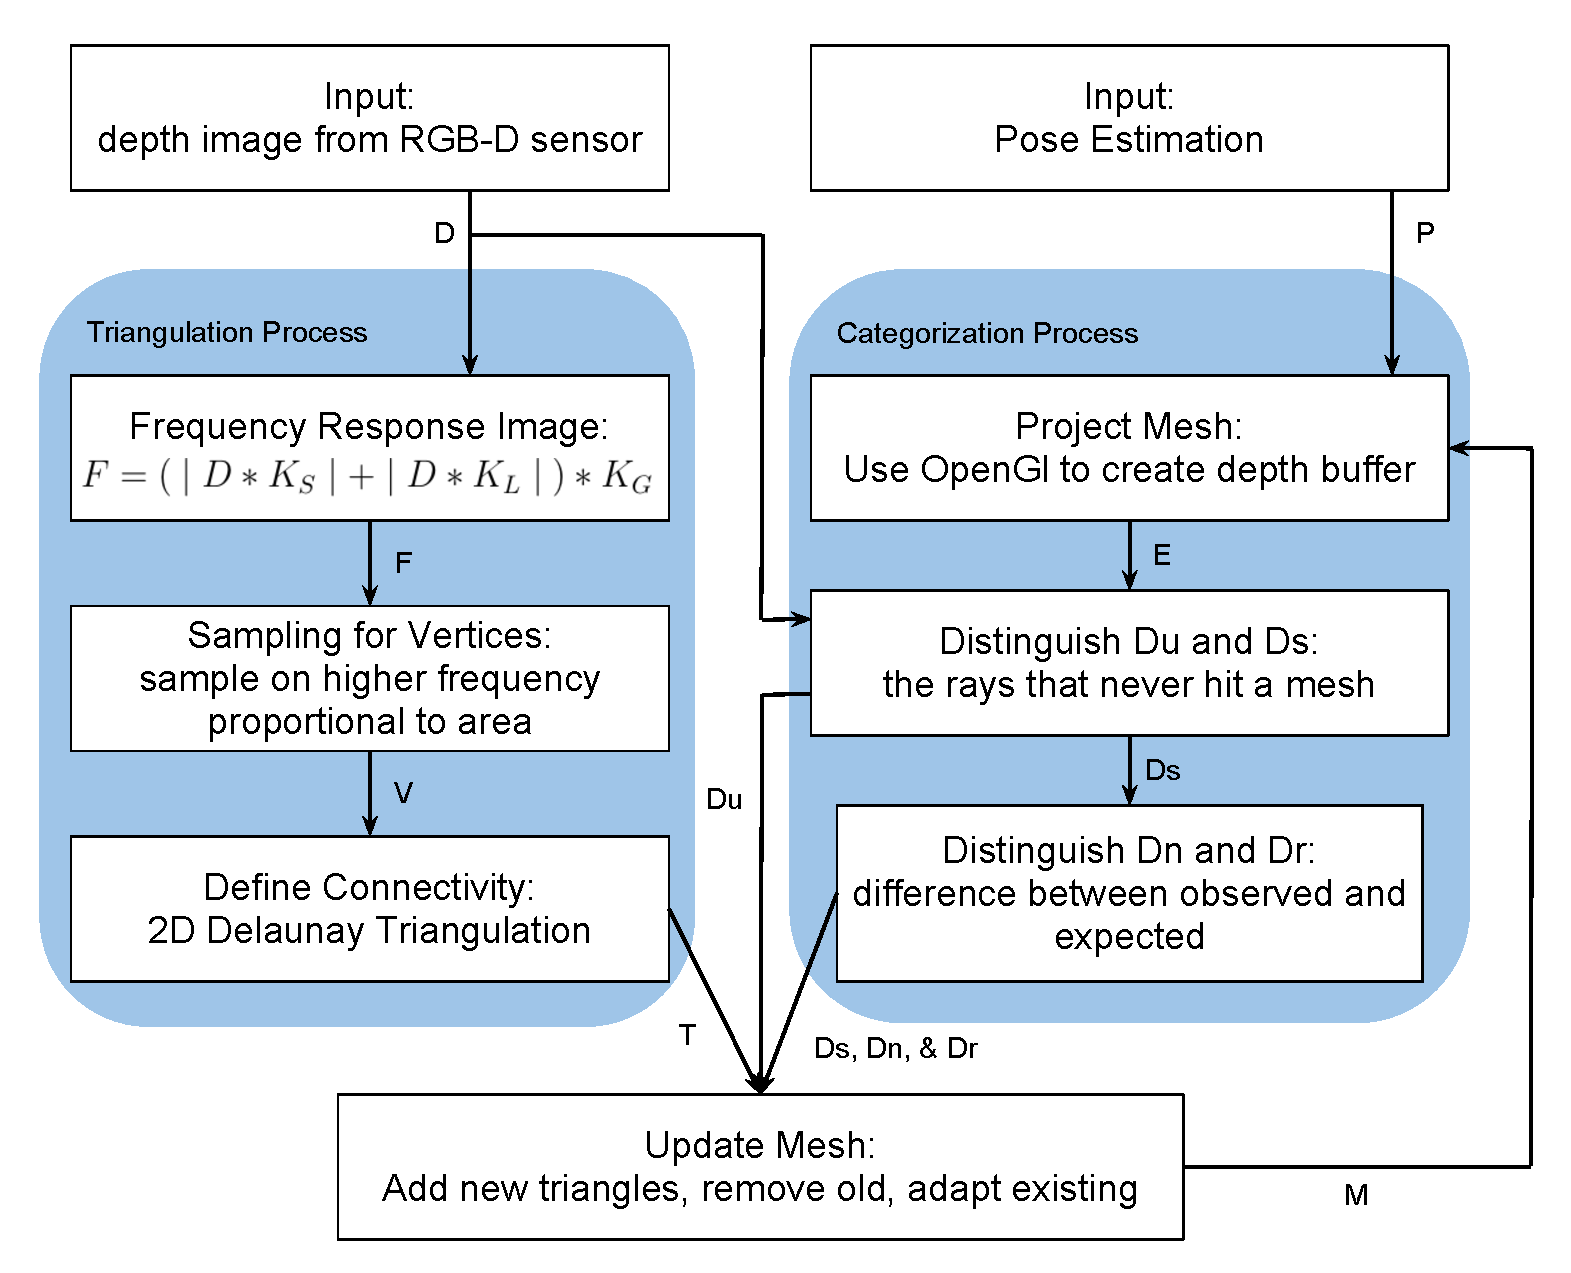
\includegraphics[height=0.6\textwidth]{SD.pdf}
  \caption{System Flow Diagram of MABDI}
  \label{fig:SD}
\end{figure}

\begin{table}[h]
\begin{center}
\begin{tabular}{|c|l|}
\hline
{\bf Variable Name} & \multicolumn{1}{|c|}{{\bf Description}} \\
\hline
\rowcolor{LightGray} $D$ & Depth image from RGB-D sensor \\ 
$F$ & Frequency response image \\
\rowcolor{LightGray} $K_S,K_L,\text{ and }K_G$ & Image convolution operators \\
$V \text{ and } C$ & Mesh vertices and connectivity of the current triangulation \\
\rowcolor{LightGray} $T$ & Current triangulation. Contains both $V$ and $C$ \\
$P$ & The known pose of the sensor \\
\rowcolor{LightGray} $E$ & Expected depth image \\ 
$D_u$ & Previously \emph{unseen} parts of $D$ \\ 
\rowcolor{LightGray} $D_s$ & Parts of $D$ which \emph{support} an existing part of
$M$ \\ 
$D_n$ & Parts of $D$ which correspond to a \emph{new} object \\ 
\rowcolor{LightGray} $D_r$ & Parts of $D$ which correspond to a
\emph{removed} object \\ 
$M$ & Current mesh \\
\hline
\end{tabular}
\end{center}
\caption{Basic description of the main variables}
\label{tab:var}
\end{table}

In the remaining sections of the Approach we will discuss the two
processes which prime the update step in detail. Finally, we will
discuss how the outputs are used to update the existing mesh map.

\subsection{Triangulation Process}

The goal of this process is to use the current depth image $D$ to estimate a
mesh of the current view of the environment. We can see a
simplified system flow chart of this process in Figure \ref{fig:SD_CT}.
Also, we can see an example of the outputs of the process using an
example input in Figure \ref{fig:O_CT}. It is important to
remember that not all of these new elements will be used in the update.
The decision of which elements from $T$ to use will be based on the
output of the Classification Process. 

\begin{figure}[h!]
  \centering
    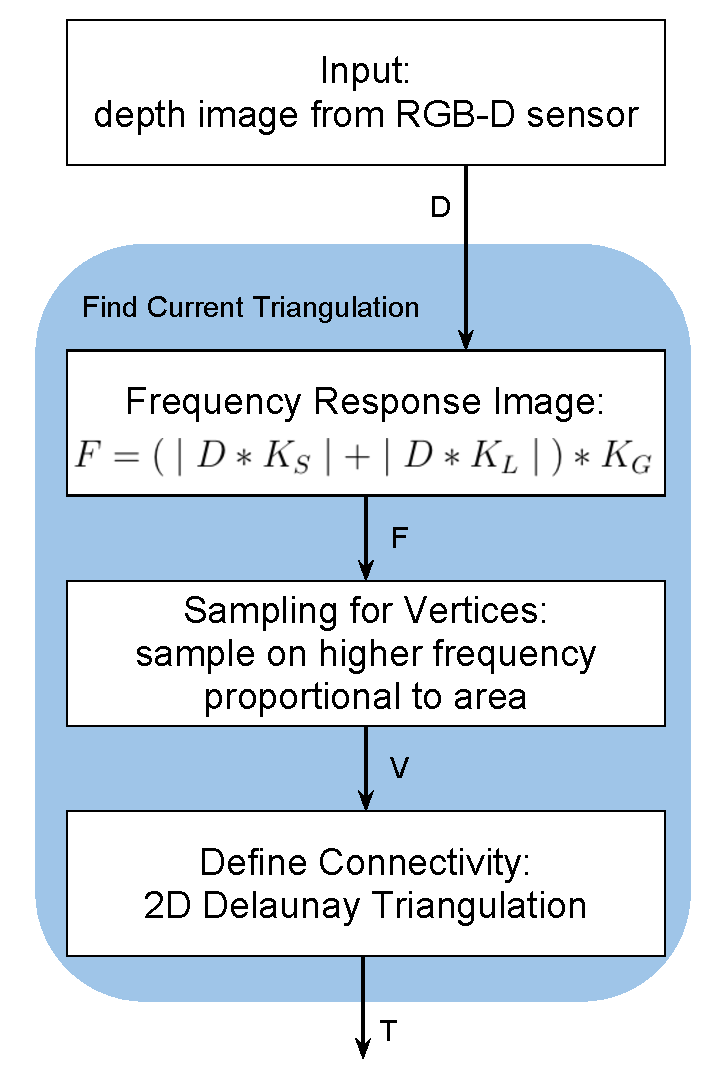
\includegraphics[height=0.4\textwidth]{SD_CT.pdf}
  \caption{Flow Diagram of Current Triangulation Process}
  \label{fig:SD_CT}
\end{figure}

\begin{figure}[h]
\centering
\subfloat[Color Image]{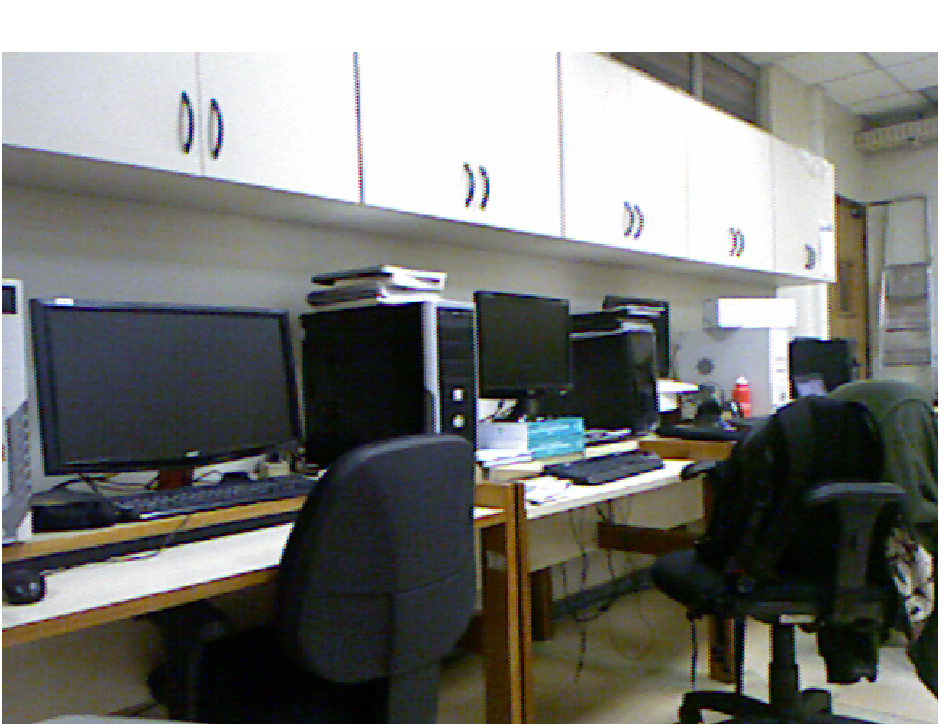
\includegraphics[width=.3\textwidth]{m_photo.pdf}} \quad
\subfloat[Depth Image $D$]{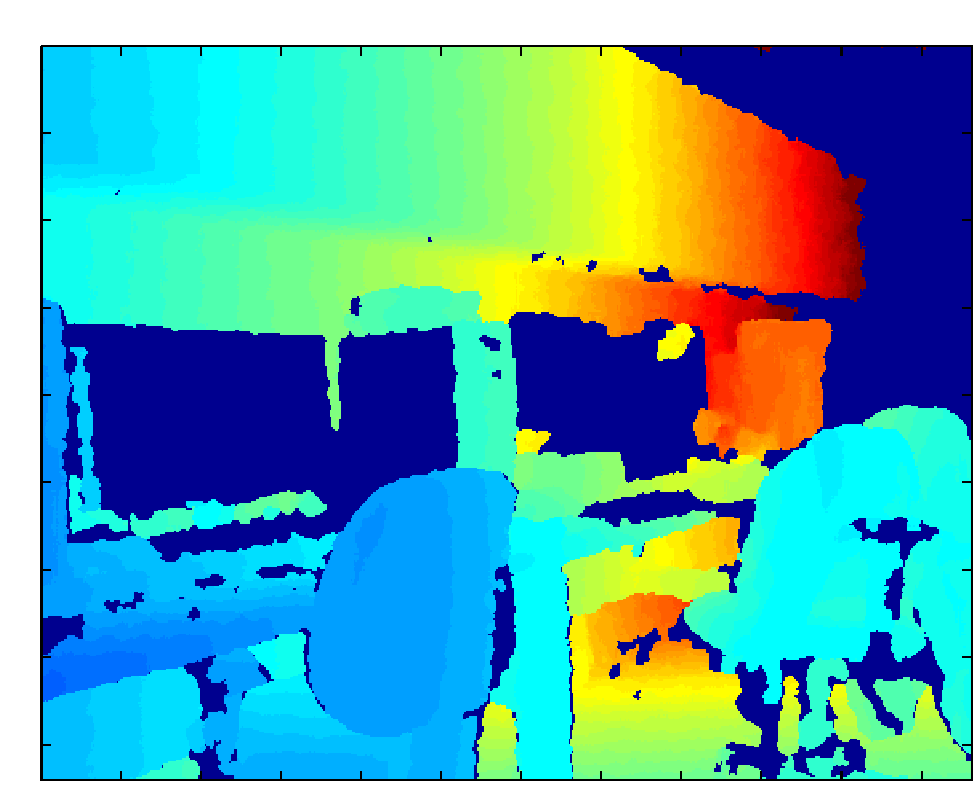
\includegraphics[width=.3\textwidth]{m_depth.pdf}} \quad
\subfloat[High Frequency Response $F$]{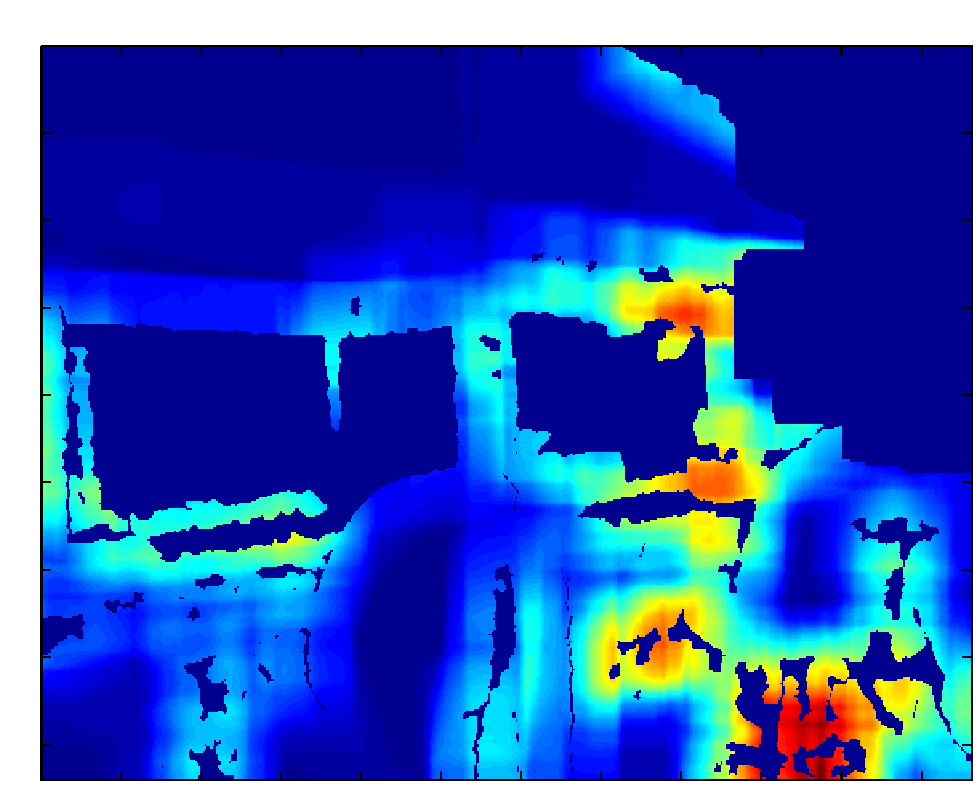
\includegraphics[width=.3\textwidth]{m_freqn.pdf}} \\
\subfloat[After Histogramming $F$]{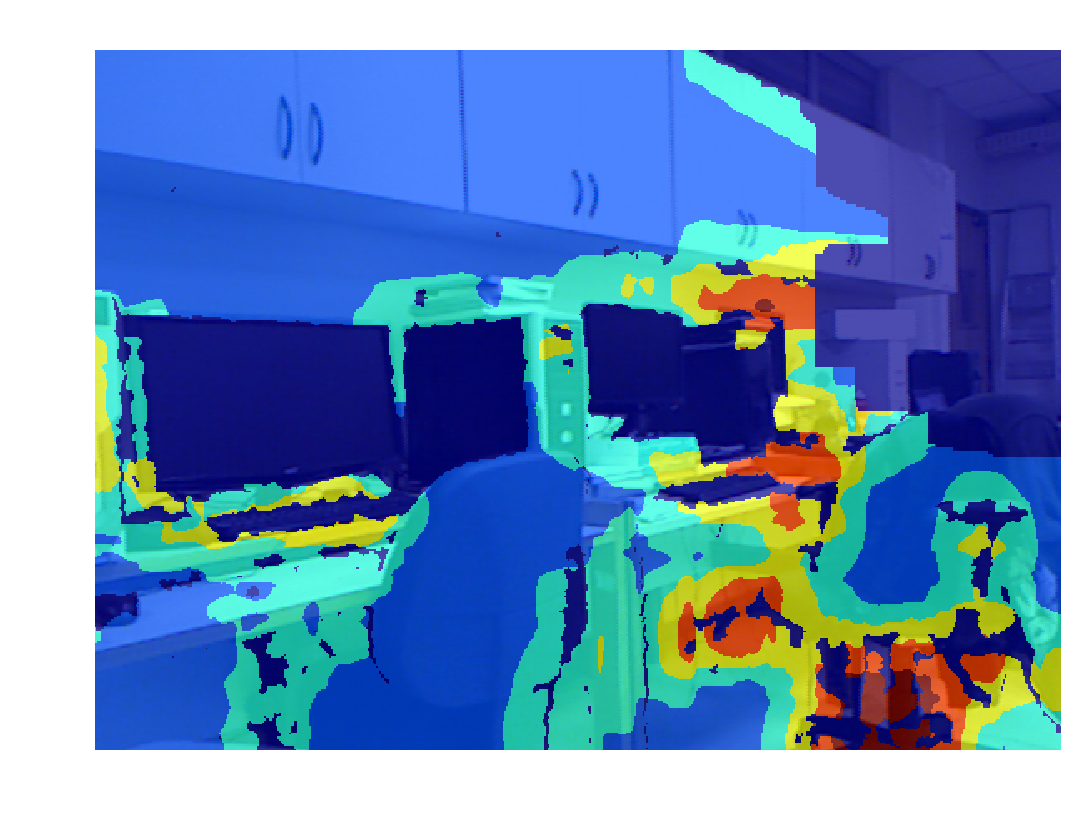
\includegraphics[width=.3\textwidth]{m_ihist.pdf}} \quad
\subfloat[Sampled Vertices $V$]{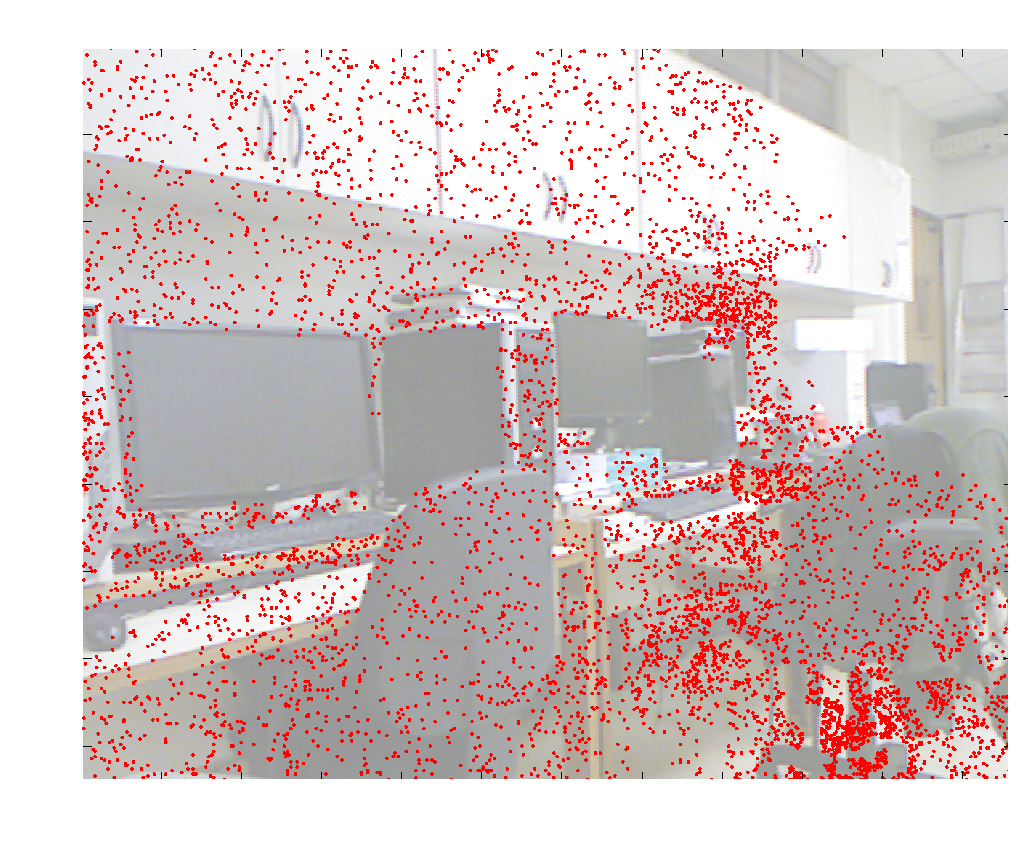
\includegraphics[width=.3\textwidth]{m_csamples.pdf}} \quad
\subfloat[Triangulation $T$]{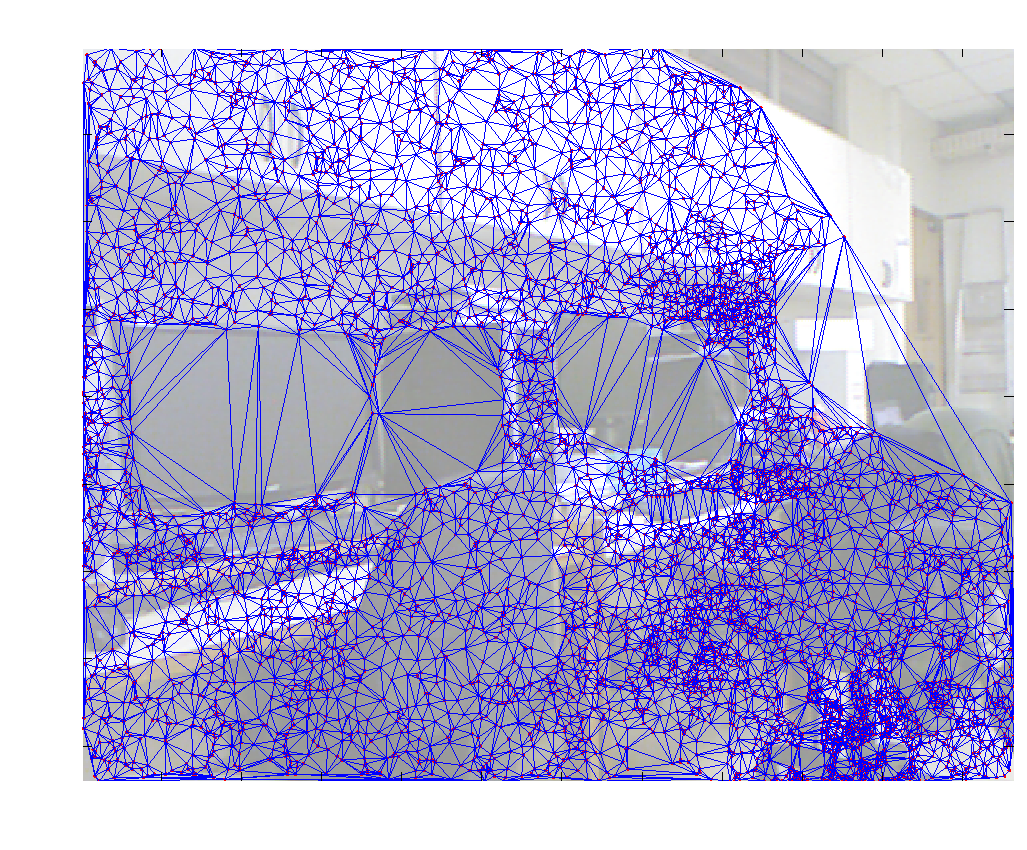
\includegraphics[width=.3\textwidth]{m_ctr.pdf}} \\
\caption{An example of the Triangulation Process. The idea is to start
with a input depth image $D$ and output a triangulation $T$ which has a
topology which is adaptive to the frequency content of the scene.}
\label{fig:O_CT}
\end{figure}

\subsubsection{Frequency Response Image}

The objective of this step is to use image processing techniques to
quickly give an estimate of the frequency content in the depth image
$D$. The end product will be an image $F$ which is the same size as $D$
and will have high values in regions with high change. In order to accomplish
this we will use a sequence of image convolutions. Equation \ref{eqn:HF}
gives the mechanics of the calculation. The Sobel operator $K_S$ is
used to give a response at corners since it is a first order
differential operator. The Laplace operator $K_L$ is used to generate a
response in areas of curvature since it is a second order differential
operator. The Gaussian operator $K_G$ is used to spread the response to the
neighboring areas.   

\begin{align}
F&=(\ \mid D \ast K_S \mid + \mid D \ast K_L \mid \ ) \ast K_G \label{eqn:HF} \\
 & K_S\text{ -- small Sobel operator}  \notag  \\
 & K_L\text{ -- small Laplace operator} \notag \\ 
 & K_G\text{ -- large Gaussian operator} \notag
\end{align}

\subsubsection{Histogram and Sample for Vertices}

The objective of this section is to use the frequency response image $F$ to
create a set of vertices $V$. These vertices will be defined as locations
in $D$. The idea is to have more vertices in regions of $D$
that have a high frequency content. In order to accomplish this, we first
define regions of similar frequency content by histogramming $F$. An
example of this histogramming can be seen in Figure \ref{fig:O_CT}d.  Next
we will probabilistically sample $F$ to define a set of vertices $V$. The
probability of each pixel being sampled is given by Equation \ref{eqn:vpr}.
The probability is calculated by the product of two different weights:
$W_F$ is based on the region of $F$ where the measurement comes from and
$W_A$ is the proportional area of that region. The result of sampling for
vertices can be seen in Figure \ref{fig:O_CT}e. In addition, because the
probability of picking each pixel as a vertex can be calculated
independently, the process is parallelizable.   

\begin{align}
p(u,v) = W_F(u,v)*W_A(u,v)
\label{eqn:vpr}
\end{align}

\subsubsection{Determine Connectivity}

Here we will use 2D Delaunay triangulation to define a connectivity
between the set of vertices $V$ found in the previous step. We are able
to define the connectivity in $\scriptstyle{\mathbb{R}}^2$ space because
the topology is conserved as we project the elements into
$\scriptstyle{\mathbb{R}}^3$.


\subsection{Classification Process}

The goal of the classification process is to use the difference between the
actual $D$ and the expected depth image $E$ to classify regions of the
depth image $D$ by the effect they will have on the model. The system flow
diagram of the classification process can be seen in Figure
\ref{fig:SD_CM}. In order to generate an expected depth image $E$ we will
use the existing mesh map $M$ and the known pose of the sensor $P$ to
create an artificial depth map of the what we expect the sensor to see $E$.
We can then use image differencing and binary blob detection to segment
regions of the depth map $D$.  

\begin{figure}[h]
  \centering
    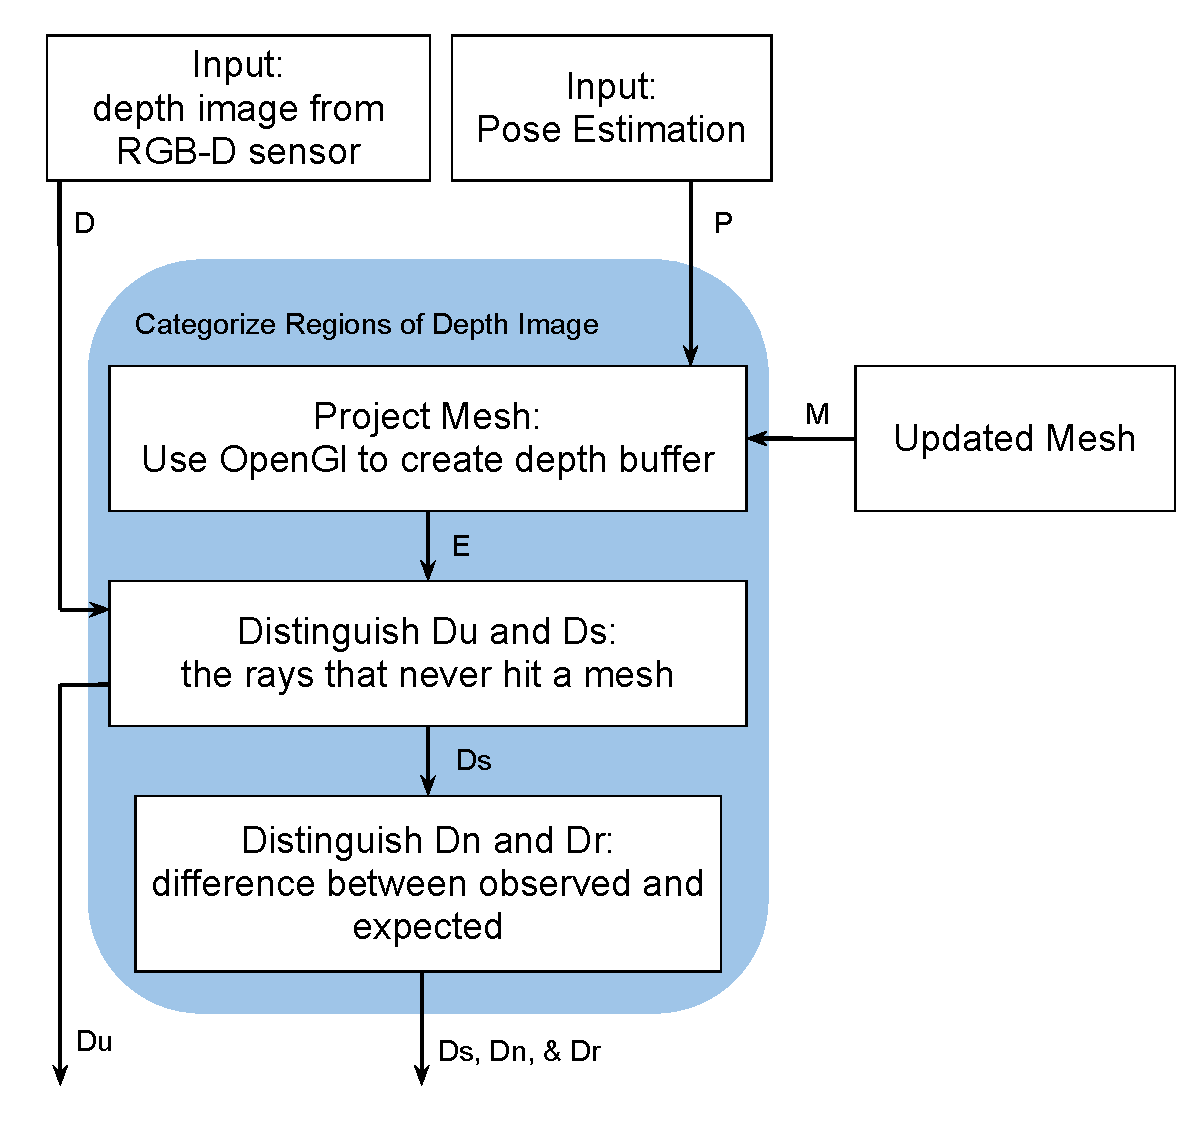
\includegraphics[height=0.4\textwidth]{SD_CM.pdf}
  \caption{Flow Diagram of Categorize Measurements Process}
  \label{fig:SD_CM}
\end{figure}

\subsubsection{Generate Expected Depth Image $E$}

We will use an existing graphics code library named OpenGL to generate an
expected depth image $E$.  A similar approach was used by Fallon et al. in
\cite{Fallon2012}.  Figure \ref{fig:proj} is a figure from Fallon's paper
which gives a clear idea of the proposed method. The procedure will be to
give the existing mesh model $M$ and the current pose $P$ to OpenGL and
render a depth buffer. It is possible to define the intrinsic parameters of
the sensor to match the actual sensor. Figure \ref{fig:proj}a and
\ref{fig:proj}b give an example of this process.  Figure \ref{fig:proj}b
represents the output of this step being the expected depth image $E$. In
addition, Figure \ref{fig:proj}d gives an example of $D$ and also in Figure
\ref{fig:proj}d we can see a RGB image of the scene.    

\begin{figure}[h]
  \centering
    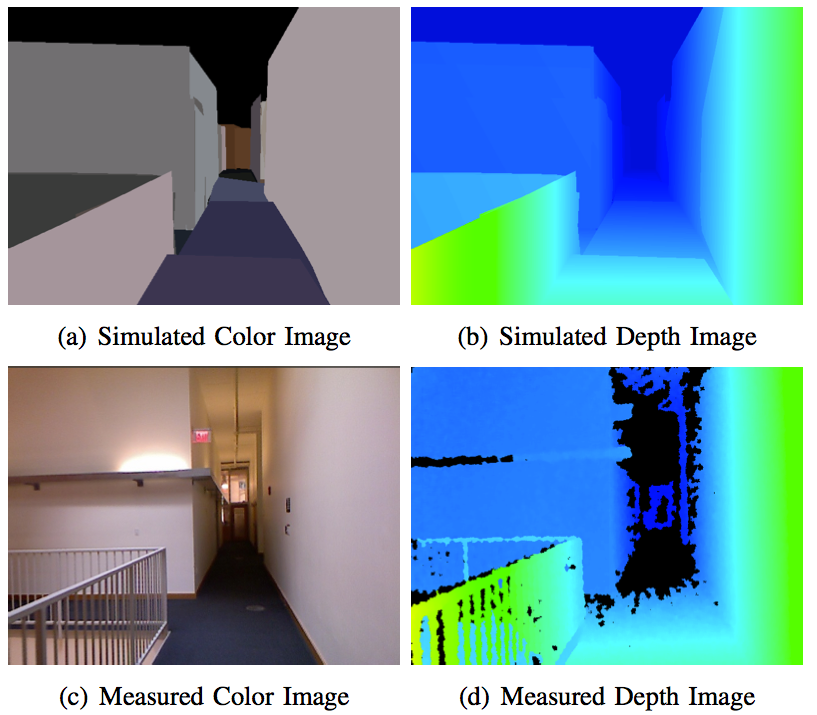
\includegraphics[height=0.6\textwidth]{m_proj.png}
  \caption{Work from \cite{Fallon2012} which generates an expected depth image $E$
in the same way as the proposed method.}
  \label{fig:proj}
\end{figure}

\subsubsection{Find Unknown Parts of the Scene}

The objective of this step is to determine regions of the depth image
$D$ which correspond to areas of the environment that have never been
seen before. This will be accomplished by finding regions of $E$ that
have no measurement. This occurs when the ray traced through the pixel
never hits a mesh element. Regions which are unseen will be designated
as $D_u$ and the rest will be designated as $D_s$. 

\subsubsection{Find New and Removed Objects}

The objective of this step is determine if measurements from the known
region of the environment $D_s$ correspond to new $D_n$ or removed $D_r$
objects in the scene. If they do not belong to $D_n$ or $D_r$ then they
support an existing surface in the mesh map. Essentially they belong to
a supporting region $D_s$ until proven otherwise. In order to prove
otherwise we will use image differencing between the expected $E$ and
the seen parts of the environment $D_s$. We will threshold the
differenced image with $-\epsilon$ and $+\epsilon$ to make two distinct
binary images. Blob analysis will then be run on this image to determine
$D_n$ and $D_r$.  

\subsection{Update Mesh}

This is the last and most important step of MABDI. Here
we will combine the triangulation $T$ found in the Triangulation Process
and the regions $D_u$, $D_s$, $D_r$, and $D_n$ found from the
Classification Process to efficiently update the existing mesh map $M$. 

\subsubsection{Add or Remove Mesh Elements}

If the measurements in $D$ correspond to new objects $D_s$ or to unseen
parts of the environment $D_n$, new mesh elements will need to be added.
The new elements will come from the triangulation defined in $T$. In
order to successfully merge the new elements with the existing mesh $M$
the bordering vertices of the region will need to be found and stitched.
It is proposed that this merging operation can be done in $D$. 

If the measurements in $D$ correspond to removed objects $D_r$, then the
elements are removed from $M$. This is done by marking the vertices
within the $D_r$ region and deleting them and their connections.  

\subsubsection{Adapt Existing Mesh}

Regions of the depth map which support an existing surface of the mesh
model will be used to adapt the mesh in order to better approximate the
real world. The idea of this process can be seen in Figure \ref{fig:AM}. In
this figure the real world is represented by the blue surface in Figure
\ref{fig:AM}a. The red dots represent the measurements from $D$. The mesh
$M$ is represented by the green surface. In the figure we see a single
vertex being adjusted. In Figure \ref{fig:AM}b a set of planes are defined
at the surrounding vertices and another plane is defined through the
measurements which correspond to this particular vertex. This neighborhood
of measurements will be found by defining a neighborhood in $D$. In Figure
\ref{fig:AM}c the vertex is adjusted. This adjustment will be done by
applying the Quadratic Error Measurement (QEM). The QEM will adjust the
vertex to minimize the distance between all planes which were found in
Figure \ref{fig:AM}b.    

\begin{figure}[h]
\centering
\subfloat[Vertex with neighboring measurements]{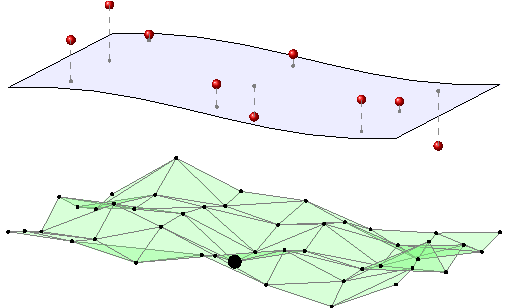
\includegraphics[width=.3\textwidth]{AM1.pdf}} \quad
\subfloat[Fitting a plane at neighboring vertices and through
neighborhood of measurements]{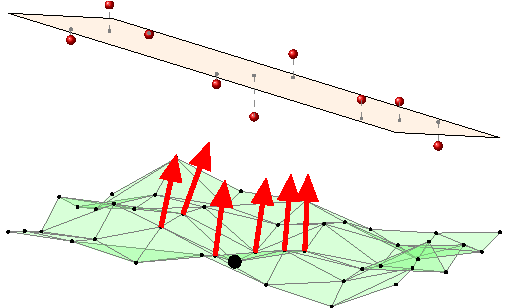
\includegraphics[width=.3\textwidth]{AM2.pdf}} \quad
\subfloat[Movement of vertex based on QEM]{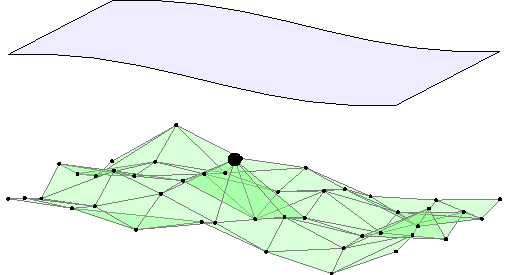
\includegraphics[width=.3\textwidth]{AM3.pdf}} \\
\caption{This shows the process of adapting a single vertex with new
measurements. }
\label{fig:AM}
\end{figure}

\section{Validation}
\label{ch:validation}

In order to evaluate and quantify the effectiveness of MABDI, a series of
experiments will be run in simulation.  The reason for validating through
simulation is that we will have control of all aspects of the experiment.
In addition, we will have a known position of the sensor in a known
environment. This will allow us to quantitatively measure our error. Figure
\ref{fig:Sim} gives an idea of how the simulation will be accomplished. We
will use a 3D modeling software named blender to create the environment and
save it to a .ply file. Then, we will use OpenGl to open the .ply file and
simulate readings from an RGB-D sensor. Finally, we will port these
measurements to Matlab where MABDI will be
developed and tested. 

\begin{figure}[h]
\centering
\subfloat[Define geometry in Blender]{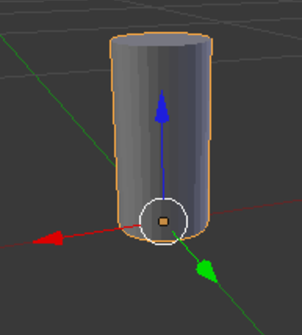
\includegraphics[width=.25\textwidth]{Sim1.pdf}} \quad
\subfloat[Render depth map in OpenGl]{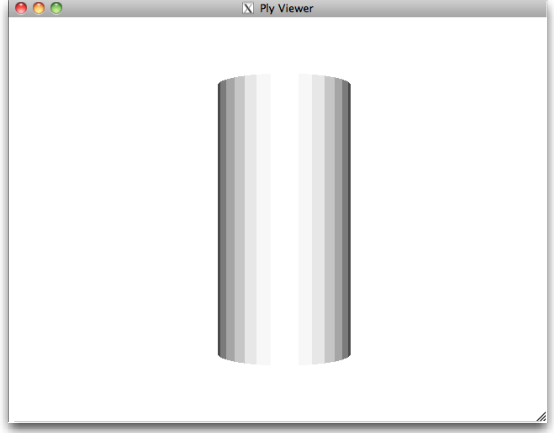
\includegraphics[width=.25\textwidth]{Sim2.pdf}} \quad
\subfloat[Export depth image to Matlab]{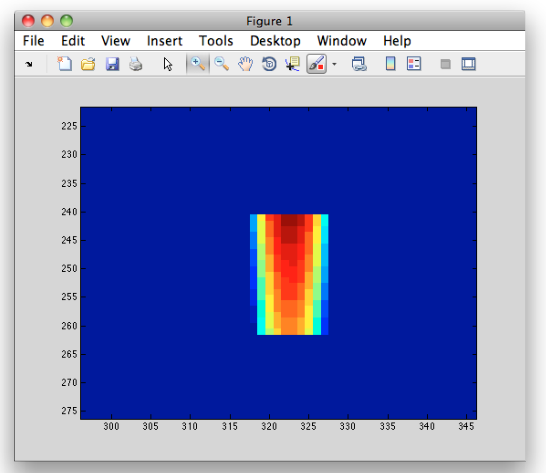
\includegraphics[width=.25\textwidth]{Sim3.pdf}} \\
\caption{The steps of the simulation pipeline. The pipeline will allow
us to simulate a RGB-D sensor viewing a known environment with a known
pose.}
\label{fig:Sim}
\end{figure}

With this simulation pipeline we can design a set of experiments that will
sequentially test the abilities of MABDI. The idea
will be to start with the easiest tests first in order make sure the system
can map the environment under the most ideal conditions. Then, each
subsequent experiment will aim to test a particular part of the system. By
testing in this sequential manner we will be able to isolate and
troubleshoot problematic parts of the system. Consequently, we will gain
greater insight on the behavior of the system as a whole and the final
system will be robust. The last experiment will test the robustness of the
system with real world data. The following lists the proposed experiments
and briefly describes the intention behind each experiment. For discussion
purposes we can envision an environment which is made of a table and a can
on the table. 

\begin{enumerate}
\item Static scene; static object; static sensor \\
Here we will test the system under the most ideal conditions. We want to
see that the system will categorize all measurements as $D_S$ after the
initial mesh is created. We will also test the ability of the system to
adapt the current mesh over time.  
\item Static scene; static object; dynamic sensor \\
Here the sensor will move in the environment. For example, we can have it
pan across the table by 1 meter. We want the system to recognize
measurements which are from unseen parts of the environment and categorize
them as $D_U$. Also, we want new elements to be added in unknown regions
using the triangulation $T$ from the Triangulation Process.  
\item Dynamic scene; static object; static sensor \\
This experiment will test the ability of the system to detect new and
removed objects. We will do this by spontaneously adding and removing a
second object in the scene such as another cup on top of the table. We will
be looking for the system to successfully categorize the measurements as
either $D_N$ or $D_R$. We will then test the ability of the system to
quickly remove or add the corresponding mesh elements from the current
mesh. 
\item Dynamic scene; dynamic object; static sensor \\
This experiment will also test the ability of the system to react to new or
removed object. However, the object will be moved into place over time. This
will be a much more thorough testing of the Categorization Process and the
ability to quickly add and remove elements. 
\item Dynamic scene; dynamic object; dynamic sensor \\
This experiment will test the entirety of the system in simulation. We can
have the sensor circle the table while new elements are being added and
removed. 
\item Real world data \\ 
This test will show the ability of the system to work with real world data
from a RGB-D sensor. We will make use of an open source data set which is
complete with pose information. 
\end{enumerate}

\section{Tasks}
\label{ch:tasks}

There are six major phases which will need to be completed for this
research. The following sections will list the steps which must be
completed for each phase. 

\subsection{Simulation Pipeline}

\begin{itemize}
\item Model all needed environments and object in Blender.
\item Simulate a RGB-D sensor viewing the environments using OpenGL.
\item Read in the simulated sensor output to Matlab.   
\end{itemize}

\subsection{Triangulation Process}

\begin{itemize}
\item Calculate frequency response image $F$
\item Sample $F$ to obtain vertices $V$
\item Triangulate vertices to obtain $T$
\end{itemize}

\subsection{Classification Process}

\begin{itemize}
\item Generate expected $E$ from current mesh $M$
\item Image differencing and blob analysis
\end{itemize}

\subsection{Map Update}

\begin{itemize}
\item Adaptation procedure
\item Add/remove elements
\end{itemize}

\subsection{Experiments}

\begin{itemize}
\item Run validation experiments 1-6 as discussed in the Validation section. 
\end{itemize}

\section{Gantt Chart}
\label{ch:ganttchart}

In order to complete this work it will be necessary to plan the completion of
the major tasks which were listed in the Tasks section. Figure \ref{fig:GC}
shows a Gantt Chart with the deadlines for each of the 5 major tasks and
also shows the time needed for writing the Thesis. The Simulation Pipeline
will be created first in order to have a database which will be used in
code development of the other processes. It is important to note that some
prior code development has been started and is represented by the gray
portion of the task bars in Figure \ref{fig:GC}. I plan to defend my thesis
by July 8th, 2013.    

\begin{figure}[h]
\begin{center}
\begin{ganttchart}[y unit title=0.4cm,
y unit chart=0.7cm,
vgrid,hgrid, 
title label anchor/.style={below=-1.6ex},
title left shift=.05,
title right shift=-.05,
title height=1,
bar/.style={fill=gray!50},
incomplete/.style={fill=white},
progress label text={},
bar height=0.7,
group right shift=0,
group top shift=.6,
group height=.3,
group peaks={}{}{.2}]{14}
%labels
\gantttitle{April}{4}
\gantttitle{May}{4}
\gantttitle{June}{4}
\gantttitle{July}{2}
\\
%tasks
\ganttbar[progress=80]{Simulation Pipeline}{1}{2} \\
\ganttbar[progress=75]{Triangulation Process}{2}{4} \\
\ganttbar[progress=0]{Classification Process}{4}{7} \\
\ganttbar[progress=0]{Map Update}{7}{9} \\
\ganttbar[progress=10]{Validation}{9}{12} \\
\ganttbar[progress=0]{Write Thesis}{12}{14} \\
\end{ganttchart}
\end{center}
\caption{Gantt Chart}
\label{fig:GC}
\end{figure}

\section{Committee}
\label{ch:committee}

The committee members consist of:

\begin{itemize}
\item Dr. Ron Lumia - Department of Mechanical Engineering 
\item Dr. Rafael Fierro - Department of Electrical Engineering
\item Dr. Robert Anderson - Sandia National Laboratories 
\end{itemize}

\pagebreak

%\begin{footnotesize}
\bibliographystyle{ieeetr}
\bibliography{library}
%\end{footnotesize}

\end{document}


